\chapter{Producto. Análisis Teórico-Computacional}\label{chapter:proposal}

HCVet es una App movil para gestionar y administrar histórias clínicas de mascotas, donde los usuarios pueden tener registros de cada consulta que se ha hecho su mascotas,saber sus padecimientos y antecedentes de forma rápida y precisa. Esto es de mucha ayuda a la hora de atender a su mascota en las visitas al veterinario,y tambien para tener conciencia de los cuidados y la atención que se le debe dar.

Se tiene una Application Programming Interface(API) para manejar la sincronizacion entre los clientes, el producto al que se refiere esta tesis es precisamente a la API. La primera vez que una persona va a usar la app debe registrarse, por tanto debe conectarse al servidor, este le asignara dos espacios para registrar dos mascotas, en caso de querer más debera realizar una suscripción.

La App cuenta con varias vistas para distintos tipos de consulta que se pueda hacer su mascota como patología, radiología, una visita médica regular, una cirugía, ect. Cada una cuenta con una serie de datos que se pedirán para llenar segun el tipo de consulta. Los usuarios también podrar asignar a otros como \textbf{encargados} de sus mascotas, para que estos también puedan registrar consultas sobre  las mascotas de otros dueños, por ejemplo un familiar o amigo.

Una de las cosas mas particularas que tiene este software es que está pensado para que casi todas sus funcionalidas se puedan hacer fuera de líena (offline), o sea, sin estar conectado a internet. Se pensó de esta forma para evitar la total dependencia de un servidor, ya que a algunas personas les puede ser un poco difícil el acceso a la red. Debido a esto se tuvieron que hacer algunas modificaciones en la estcutura del proyecto, para que el servidor pudiera hacer un proceso de sincronizacion, correcto y eficiente.Los datos de todos los usuarios estarán en el servidor, pero tambien cada uno tendrá sus datos particulares en una base de datos local en su móvil. 

\section{Casos de Uso}
El proceso de sincronización cuenta con las siguientes funcionalidades o casos de uso, que estas si requieren de conexión a internet :
\begin{itemize}
	\item Subir datos al servidor :
	
	Los nuevos datos generados se subirán al servidor. Esto se realizo para tener una centralizacion de los datos, y de alguna forma una copia de seguridad de los mismos, en caso de perdida. También sirve para el proceso de sincronización en usuarios que tengan masctas en común, al tener esos datos en el servidor, proveerá esos datos a los usuarios que le sean requeridos.
	
	\item Bajar datos del Servidor :
	
	Todos los datos que hayan sido subidos al servidor, de todas las mascotas que el usuario sea dueño serán agregados a la base de datos local. Está funcion mantiene actualizados los datos de cada usuario, por ahora solo agrega daatos, en un futuro se pudiara mejorar esta acción para que también actualice y elimine datos, que este proceso puede ser bastante complejo. 
	
	\item Asignar encargado :
	
	Se le notificará al servidor que un usuario ha sido asignado como encargado de una nueva mascota. Esta funcion es necesaria, para que el servidor pueda proveer de los nuevos registros tanto a los dueños como a los encargados.
	
		\item Desasignar encargado :
	
	Se le notificará al servidor que un usuario ha dejado de ser  encargado de una mascota. A la vez que un cliente deje de tener relacion con la mascota, se deberá tener encuenta para que no lleguen datos innecesarios a la hora de sincronizar   
\end{itemize}

  \section{Propuesta de Arquitectura}
  
  Se tuvieron en cuenta varias arquitecturas, todas varían un poco en sus detalles, pero son bastante parecidas, ya que tienen un objetivo en común, la separación de obligaciones dividiendo el software en capas. Valorando la capacidad de extender la solución así como la testeabilidad de la misma en un futuro.
  
  \subsection{Clean Architecture}
  Clean Architecture ,popularizada por Robert Cecil Martin, es una arquitectura de capas, y
  en estas arquitecturas las capas se colocan de forma horizontal, donde una capa solo puede depender
  de otra que esté por debajo de ella, nunca por encima. Puede ver la figura \ref{fig:clean_architecture} que muestra a través
  de un diagrama la estructura y el flujo de esta arquitectura de forma general.\brackcite{cleanArchitecture}
  
\begin{figure}
	\centering
	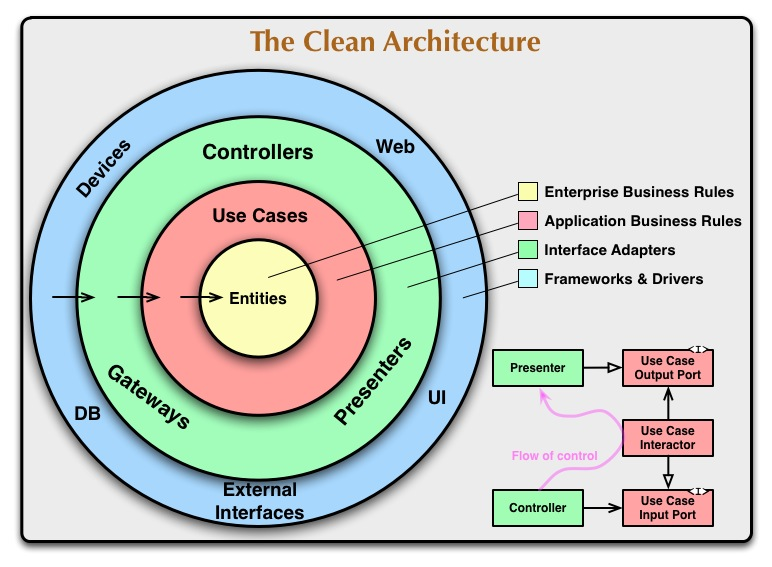
\includegraphics[width = 14cm]{MainMatter/CleanArchitecture.jpg}
	\caption{Diagrama de Clean Architecture }
	\label{fig:clean_architecture}
	
\end{figure}	
\newpage
\subsubsection{Regla de dependencia}
  
  Los círculos concéntricos representan diferentes áreas de software. En general, cuanto más avance, mayor será el nivel del software. Los círculos exteriores son mecanismos. Los círculos internos son políticas.
  
La regla primordial que hace que esta arquitectura funcione es la regla de dependencia. Esta regla dice que las dependencias del código fuente solo pueden apuntar hacia adentro. Nada en un círculo interior puede saber absolutamente nada sobre algo en un círculo exterior. En particular, el nombre de algo declarado en un círculo exterior no debe ser mencionado por el código en un círculo interior. Eso incluye, funciones, clases. variables, o cualquier otra entidad de software nombrada.


Del mismo modo, los formatos de datos utilizados en un círculo exterior no deberían ser utilizados por un círculo interior, especialmente si esos formatos son generados por un marco en un círculo exterior. No queremos que nada en un círculo exterior impacte en los círculos interiores. \brackcite{cleanArchitecture}



\subsubsection{Uso de Arquitectura}
Para la implementación de esta arquitectura la aplicación se dividirá en las 3 capas descritas a continuación:

\begin{itemize}
	\item \textbf{Core}: La capa más interna, no es susceptible a cambios en otras capas, es totalmente independiente. Esta contiene la lógica de negocio, los objetos de uso general en la aplicación(entidades),el mapeo de las entidades, definición de interfaces a implementar tanto en esta capa como en las que la envuelven.
	
	\item \textbf{Infrastructure}: : La capa referente a datos, contiene las funciones correspondientes al acceso a base de datos(BD). Se subordina a las peticiones de la capa de dominio por medio de los
	Repositorios que implementan como acceder a los datos.Contiene los servicios y repositorios para proever datos a las capas más externas.
	
	\item \textbf{API}: Expone los end-points de la aplicación, que son las funcionalidades explicadas anteriormente, esta es la capa mas externa. Aquí se convierten los datos  a la forma más conveniente para cualquier marco de persistencia que se esté utilizando. Ningún código dentro de este círculo debería saber nada sobre la BD.
	
\end{itemize}


\subsection{Modelo de Datos }


  

